\section{Modelo físico}
\subsection{Prueba de concepto}

Se construyó un péndulo simple empleando 
el kit de construcción de LEGO Mindstorms.
El uso de este kit presenta varias características
útiles para el estudio del sistema:
\begin{itemize}
 \item Unidad de computación integrada y programable.
 \item Modularidad de sus piezas.
 \item Facilidad de ensamble.
 \item Motores de corriente directa incluyen 
 codificadores rotatorios para retroalimentación.
\end{itemize}

\subsection{Análisis de video}

El modelo construido se empleó para hacer un análisis 
de su movimiento mediante el software de 
\emph{Tracker}\footnote{\url{https://www.physlets.org/tracker/}}.
Tracker es un progrma \emph{open-source} de análisis de 
video y modelado de ecuaciones, 
enfocado para sistemas físicos.

Se grabó un video del péndulo físico para evaluar el sistema
y la prueba de concepto. 
El software es capaz de obtener mediciones sensibles para
diferentes cantidades físicas como coordenadas rectangulares
y polares.
Las figuras \ref{fig: tracker phase diagram x vx} y 
\ref{fig: tracker phase diagram y vy}
muestran los diagramas fase del péndulo físico.
Se presenta también la coordenada \emph{x}
del péndulo a través del tiempo en la figura \ref{fig: tracker time diagram x}.

\begin{figure}[hb!]
 \centering
 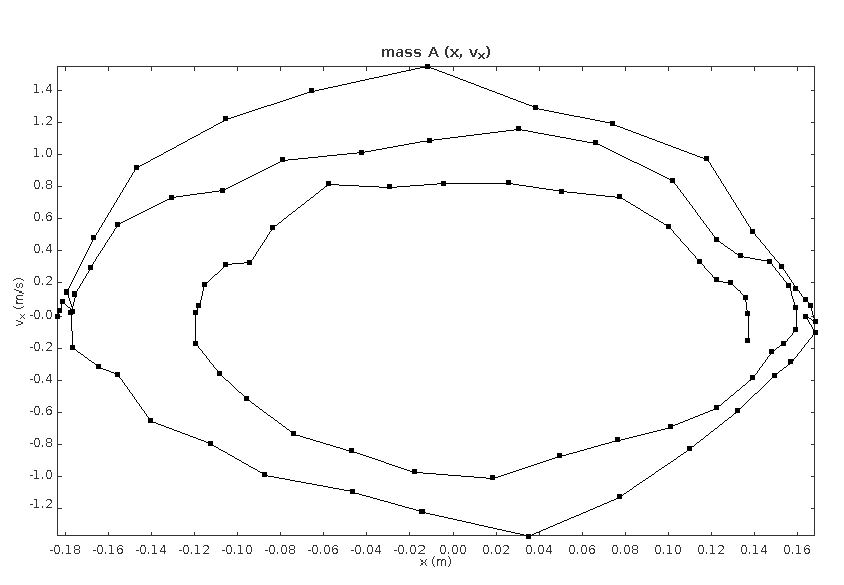
\includegraphics[scale=0.4]{./img/tracker_poc_phasediagram_x_vx.png}
 % tracker_poc_phasediagram_x_vx.png: 844x585 px, 72dpi, 29.78x20.64 cm, bb=0 0 844 585
 \caption{Diagrama de fase del modelo físico para $x$ y $\dot{x}$}
 \label{fig: tracker phase diagram x vx}
\end{figure}

\begin{figure}[hb!]
 \centering
 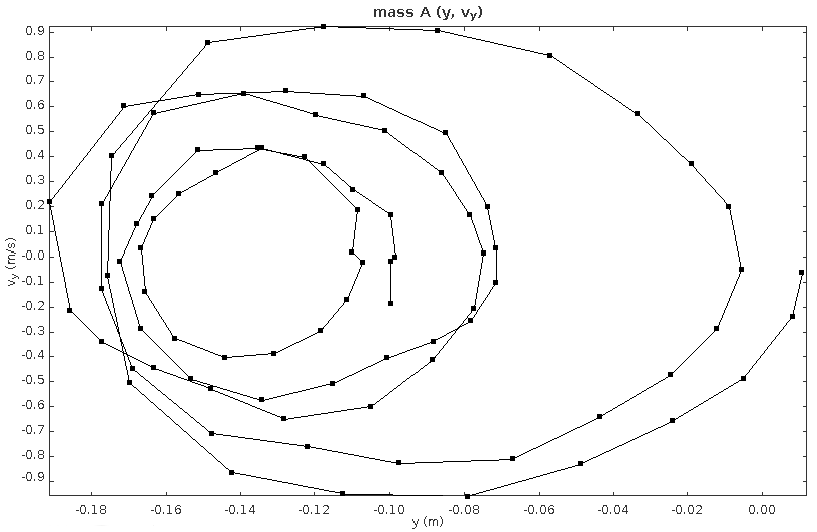
\includegraphics[scale=0.4]{./img/tracker_poc_phasediagram_y_vy.png}
 % tracker_poc_phasediagram_x_vx.png: 844x585 px, 72dpi, 29.78x20.64 cm, bb=0 0 844 585
 \caption{Diagrama de fase del modelo físico para $y$ y $\dot{y}$}
 \label{fig: tracker phase diagram y vy}
\end{figure}


\begin{figure}[hb!]
 \centering
 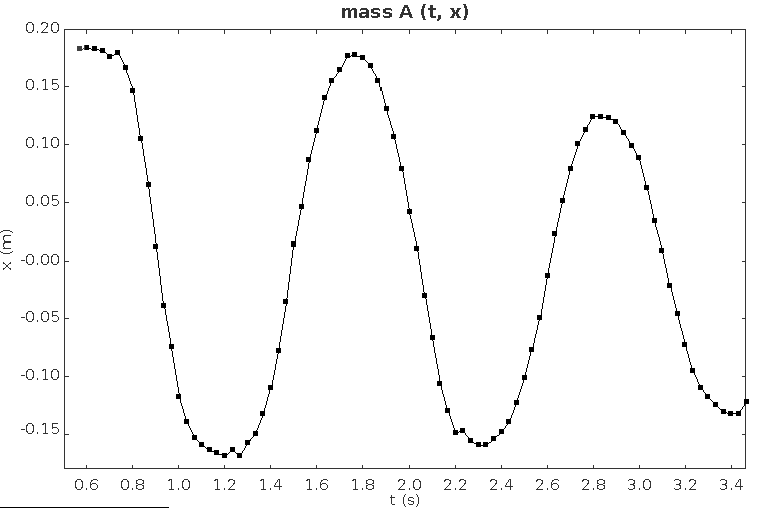
\includegraphics[scale=0.45]{./img/tracker_poc_timeplot_x.png}
 % tracker_poc_phasediagram_x_vx.png: 844x585 px, 72dpi, 29.78x20.64 cm, bb=0 0 844 585
 \caption{Diagrama de tiempo del modelo físico para $x$.}
 \label{fig: tracker time diagram x}
\end{figure}

\subsection{Mediciones físicas}

Empleando los sensores incluidos en el kit de LEGO
Mindstorms, fue posible realizar mediciones de la 
posición angular del péndulo para comparar con el
modelo matemático y el análisis de video.
La figura \ref{fig: mindstorms theta} muestra la
gráfica de mediciones de $\theta$ respecto al tiempo.
Se observa que las mediciones realizadas por el sensor
fueron afectadas por el nivel de ruido introducido 
por el mismo sensor.

\begin{figure}[hb!]
 \centering
 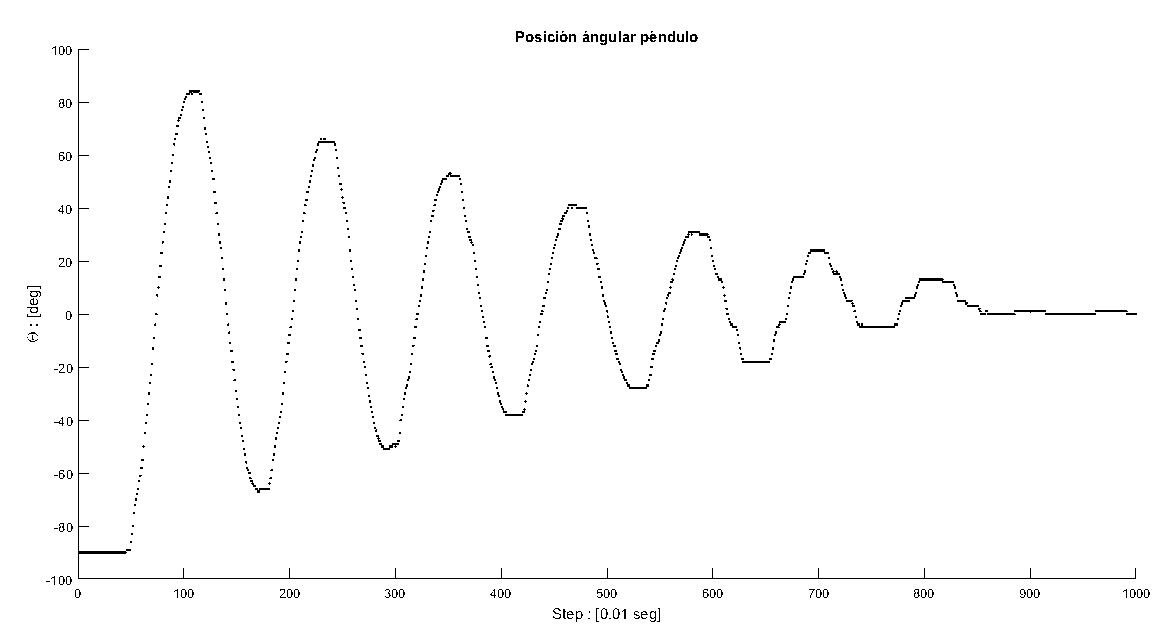
\includegraphics[scale=0.4]{../Mindstorms/Pendulin2_bw.png}
 % Pendulin2_bw.png: 1157x625 px, 96dpi, 30.61x16.53 cm, bb=0 0 868 469
 \caption{Mediciones de $\theta$ para el péndulo físico con el codificador rotatorio.}
 \label{fig: mindstorms theta}
\end{figure}


\clearpage
